\graphicspath{
    {figures_and_references/urban_surface_detection/}
    {figures_and_references/EELISA_conference/}
    {figures_and_references/footprints_paper/}
}

% \selectlanguage{english}
\renewcommand{\chapternametext}{Chapter \thechapter . Use case: Automatic building footprint instance segmentation in the 3 pilot regions}
\renewcommand{\shortchapternametext}{Chapter \thechapter . Use case: Automatic building footprint instance segmentation}

\begin{refsection}

\chapter{\chapternametext}
\

\renewcommand{\headingtextL}{}
\renewcommand{\headingtextR}{\shortchapternametext}
\begingroup
 \flushbottom
 \setlength{\parskip}{0pt plus 1fil}%
 \localtableofcontents 
\endgroup

\begingroup
 \flushbottom
 \setlength{\parskip}{0pt plus 1fil}%
 \locallistoffigures
 \locallistoftables
\endgroup


\newpage

\setcounter{section}{0} 



\FloatBarrier

\renewcommand{\sectionnametext}{Introduction}
\renewcommand{\headingtextL}{\shortchapternametext}
\renewcommand{\headingtextR}{\thesection. \sectionnametext}
\section{\sectionnametext}


Precise building digitalization is a prerequisite for seismic structural analysis, yet it remains a primary bottleneck in inventory development. Traditional semantic segmentation techniques, while effective for general land-cover classification, often fail in dense urban environments by merging adjacent structures into single, fragmented polygons \footcite{ji_fully_2019, torres_using_2023}. To maintain the geometric precision required for building-level assessment, more recent research has shifted toward instance segmentation, which assigns unique identifiers to individual structures or objects in an image \footcite{chen_large-scale_2023}.

Transformer-based architectures, such as Mask2Former \footcite{cheng_masked-attention_2022} and the Segment Anything Model (SAM) family \footcite{ravi_sam_2024}, represent the current state-of-the-art, offering high performance even with minimal or no task-specific training data \footcite{cao_feasibility_2023}. In addition to these models, two major global repositories of building footprint data are available. The first is OpenStreetMap (OSM) \footcite{haklay_openstreetmap_2008}, a community-sourced platform that relies on manual digitization by volunteers. While OSM can provide high-quality data, it is often incomplete or entirely unavailable in certain regions, as was the case in the pilot areas of this study. The second is the Microsoft Global Building Footprints dataset \footcite{microsoft_globalmlbuildingfootprints_2024}, which provides near-global coverage generated through automated computer vision models. However, while this dataset offers wide availability, it may not always achieve the specific geometric accuracy required for structural modeling in dense, high-risk urban settings.

\renewcommand{\sectionnametext}{Methodology}
\renewcommand{\headingtextL}{\shortchapternametext}
\renewcommand{\headingtextR}{\thesection. \sectionnametext}
\section{\sectionnametext}

 To prove the viability of generating large-scale exposure data at a low cost, this study explores two AI-assisted instance segmentation workflows designed to accelerate the digitalisation process.
The first approach utilizes a "one-shot" automated workflow via the Mask2Former model \footcite{cheng_masked-attention_2022}, intended for the rapid, unsupervised extraction of all structures within an orthoimage. The second approach employs an interactive workflow using SAM2 \footcite{ravi_sam_2024}, where the user provides a single point prompt inside each building. This method is designed to ensure high geometric fidelity in dense urban areas where fully automated methods often struggle.
To adapt these foundational models to the unique urban textures of the study regions, both were fine-tuned on a small, domain-specific dataset. This dataset was generated using the \textit{GeoVisionDataset} package \footcite{urena_pliego_transport-related_2025}. The dataset was randomly split into 80\% for training (82 images) and 20\% for testing (21 images). To enhance model generalisation, data augmentation techniques were applied during training, including brightness and contrast adjustments, random cropping, and horizontal and vertical flipping. The training procedure for Mask2Former followed the original implementation described in \footcite{cheng_masked-attention_2022}, while the SAM2 model was trained using the official training scripts adapted to this dataset \footcite{ravi_sam_2024}. Both models were trained for 50 epochs. Finally, the results of these localized models are benchmarked against the ground truth and the existing \textit{Microsoft Global Building Footprints} dataset \footcite{microsoft_globalmlbuildingfootprints_2024}.

In the intended practical use of this study two digitalization methods are offered depending on the required accuracy, human resources and fine-tuning possibilities:

Sequential Workflow: For large-scale projects, Mask2Former is used to generate a fully automated "first-pass" inventory. SAM2 is then employed as a refinement tool where a human operator can quickly correct or "snap" boundaries that are ambiguous. This method requires fine-tuning Mask2Former.

Alternative Workflow: In cases where high-fidelity footprints are required from the start (e.g., for specific high-risk buildings), SAM2 can be used independently with point-prompts to ensure better shape capture than the fully unsupervised Mask2Former. This method can work without any fine-tuning.

\renewcommand{\sectionnametext}{Experimental setup}
\renewcommand{\headingtextR}{\thesection. \sectionnametext}
\section{\sectionnametext}


\begin{figure}[htbp]
    \centering
    \begin{tabular}{cc}
        \begin{subfigure}[t]{0.4\linewidth}
            \centering 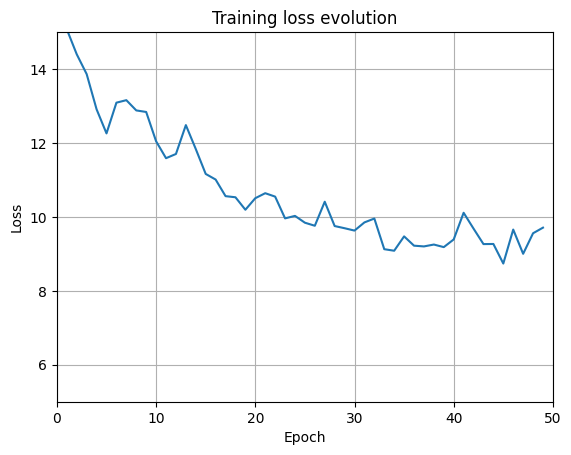
\includegraphics[width=\linewidth,height=0.8\linewidth]{figures/mask2former_train_loss.png}
            \caption{Mask2Former}
            \label{fig:mask2former_train_loss}
        \end{subfigure} & 
        \begin{subfigure}[t]{0.4\linewidth}
            \centering            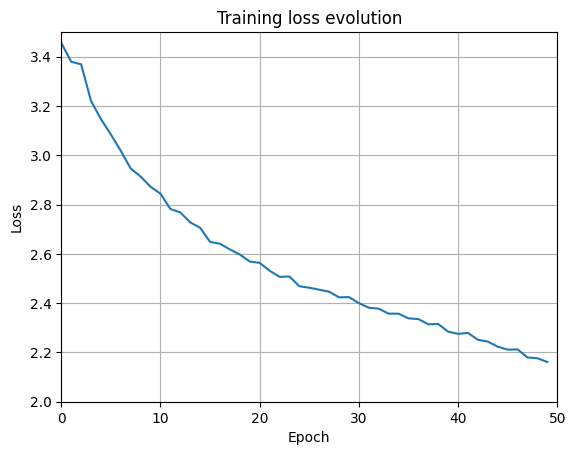
\includegraphics[width=\linewidth,height=0.8\linewidth]{figures/SAM2_train_loss.png}
            \caption{SAM2}
            \label{fig:SAM2_train_loss}
        \end{subfigure}
    \end{tabular}
    \caption{Train loss evolution of both image vision models.}
    \label{fig:train_loss}
\end{figure}

Two computer vision models, Mask2Former and SAM2, were fine-tuned and evaluated using a dataset derived from image data collected across three pilot regions. The dataset was randomly split into 80\% for training (82 images) and 20\% for testing (21 images). To enhance model generalisation, data augmentation techniques were applied during training, including brightness and contrast adjustments, random cropping, and horizontal and vertical flipping.

The training procedure for Mask2Former followed the original implementation described in \footcite{cheng_masked-attention_2022}, while the SAM2 model was trained using the official training scripts adapted to this dataset \footcite{ravi_sam_2024}. Both models were trained for 50 epochs. Notably, the Mask2Former model exhibited a rapid decrease in training loss within just 2 to 3 epochs, and overall, it trained faster and required less memory. In contrast, the SAM2 model required more memory and training time and did not reach convergence even after 50 epochs (fig \ref{fig:train_loss}).

For comparison, the Microsoft GlobalMLBuildingFootprints dataset \footcite{microsoft_globalmlbuildingfootprints_2024} was also evaluated on the same test set.

\renewcommand{\sectionnametext}{Results}
\renewcommand{\headingtextR}{\thesection. \sectionnametext}
\section{\sectionnametext}


\label{sec:res_digitalisation}
\begin{figure}[htbp]
    \centering
    \begin{tabular}{cccc}
        \begin{subfigure}[t]{0.22\linewidth}
            \centering            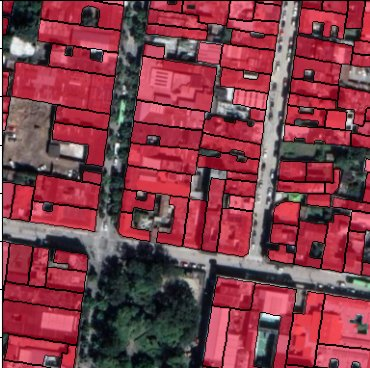
\includegraphics[width=\linewidth,height=\linewidth]{figures/guat_30cm_gt.jpg}
            \caption{Guatemala ground truth}
            \label{fig:guat_gt}
        \end{subfigure} & 
        \begin{subfigure}[t]{0.22\linewidth}
            \centering            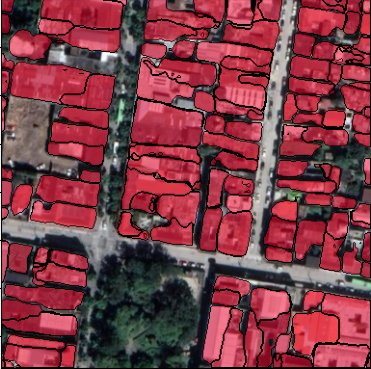
\includegraphics[width=\linewidth,height=\linewidth]{figures/mask2former_guat_30cm.jpg}
            \caption{Mask2Former}
            \label{fig:guat_m2f}
        \end{subfigure} & 
        \begin{subfigure}[t]{0.22\linewidth}
            \centering            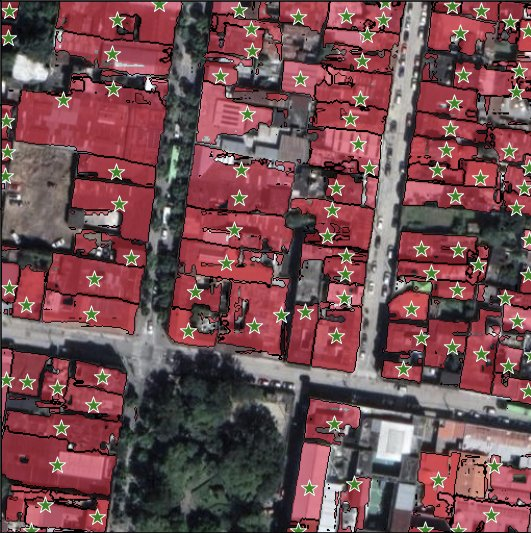
\includegraphics[width=\linewidth,height=\linewidth]{figures/SAM2_guat.jpg}
            \caption{SAM2}
            \label{fig:guat_sam2}
        \end{subfigure} & 
        \begin{subfigure}[t]{0.22\linewidth}
            \centering            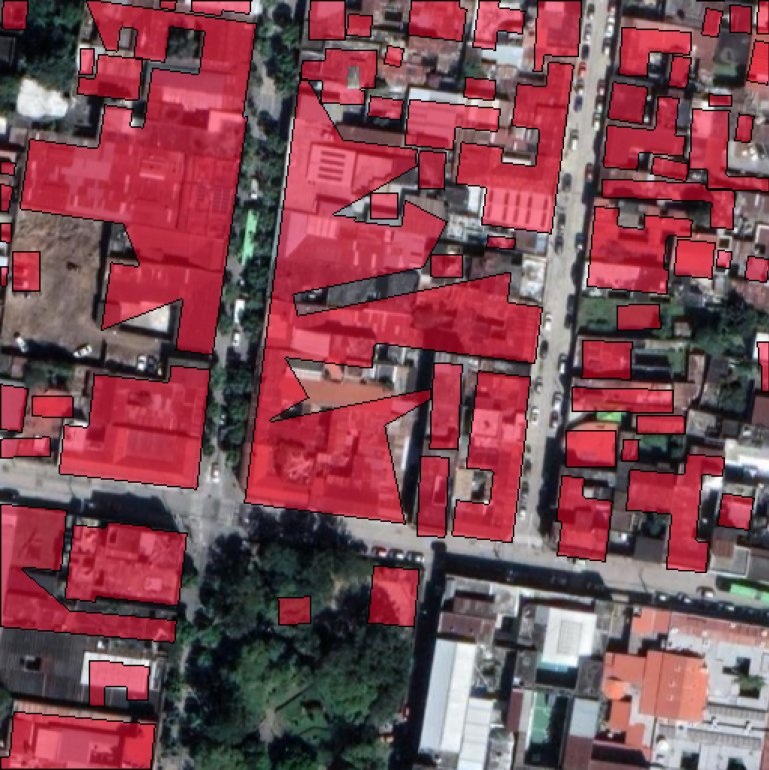
\includegraphics[width=\linewidth,height=\linewidth]{figures/guatemala_microsoft.jpg}
            \caption{Microsoft}
            \label{fig:guat_microsoft}
        \end{subfigure} \\
        \begin{subfigure}[t]{0.22\linewidth}
            \centering            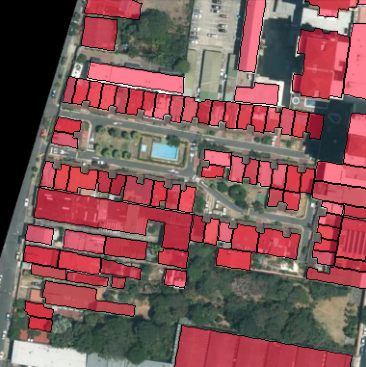
\includegraphics[width=\linewidth,height=\linewidth]{figures/sj_30cm_gt.png}
            \caption{San José ground truth}
            \label{fig:sj_gt}
        \end{subfigure} & 
        \begin{subfigure}[t]{0.22\linewidth}
            \centering            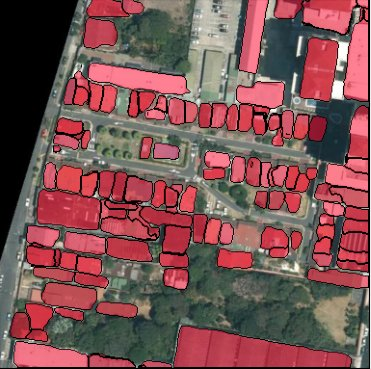
\includegraphics[width=\linewidth,height=\linewidth]{figures/mask2former_sj_30cm.jpg}
            \caption{Mask2Former}
            \label{fig:sj_m2f}
        \end{subfigure} & 
        \begin{subfigure}[t]{0.22\linewidth}
            \centering            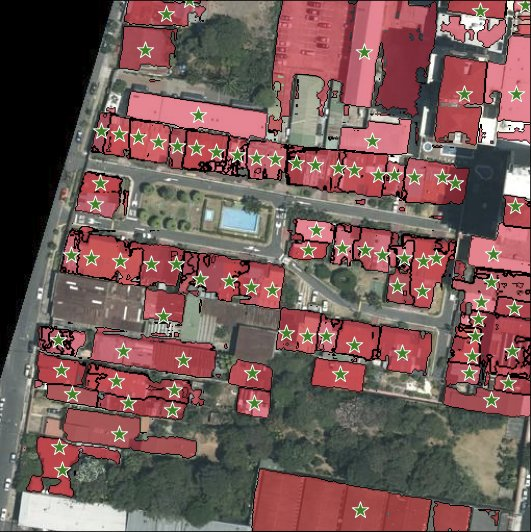
\includegraphics[width=\linewidth,height=\linewidth]{figures/SAM2_sj.jpg}
            \caption{SAM2}
            \label{fig:sj_sam2}
        \end{subfigure} & 
        \begin{subfigure}[t]{0.22\linewidth}
            \centering            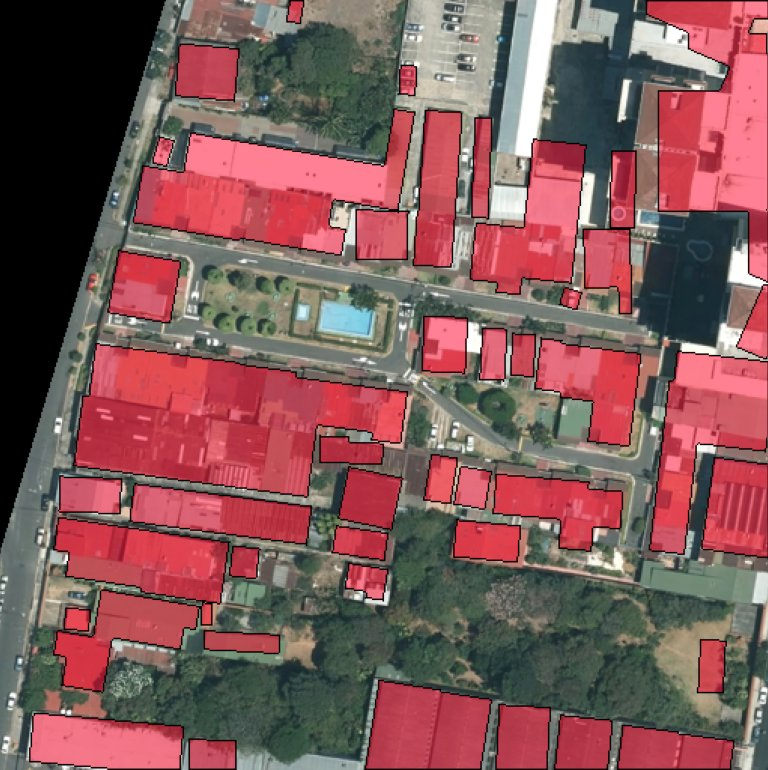
\includegraphics[width=\linewidth,height=\linewidth]{figures/san_jose_microsoft.jpg}
            \caption{Microsoft}
            \label{fig:sj_microsoft}
        \end{subfigure} \\
        \begin{subfigure}[t]{0.22\linewidth}
            \centering            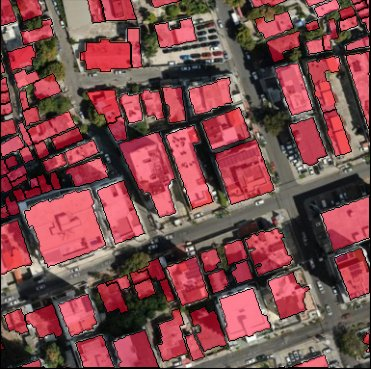
\includegraphics[width=\linewidth,height=\linewidth]{figures/sd_30cm_gt.jpg}
            \caption{Santo Domingo ground truth}
            \label{fig:sd_gt}
        \end{subfigure} & 
        \begin{subfigure}[t]{0.22\linewidth}
            \centering            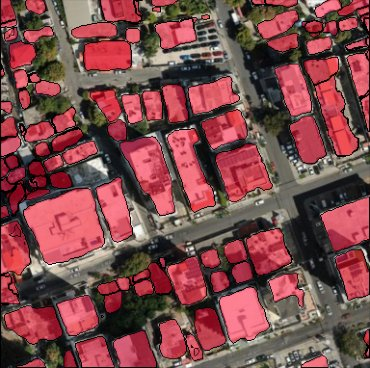
\includegraphics[width=\linewidth,height=\linewidth]{figures/mask2former_sd_30cm.jpg}
            \caption{Mask2Former}
            \label{fig:sd_m2f}
        \end{subfigure} & 
        \begin{subfigure}[t]{0.22\linewidth}
            \centering            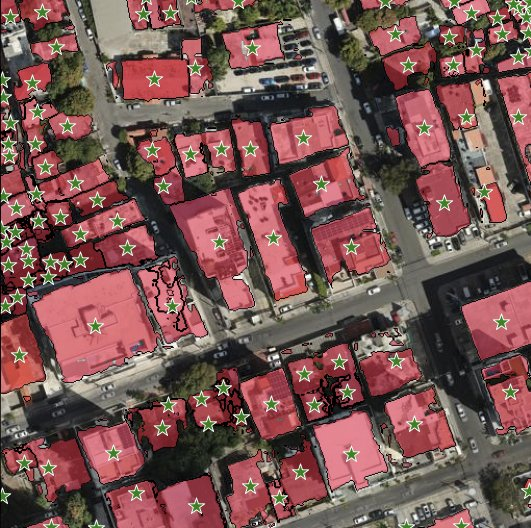
\includegraphics[width=\linewidth,height=\linewidth]{figures/SAM2_sd.jpg}
            \caption{SAM2}
            \label{fig:sd_sam2}
        \end{subfigure} & 
        \begin{subfigure}[t]{0.22\linewidth}
            \centering            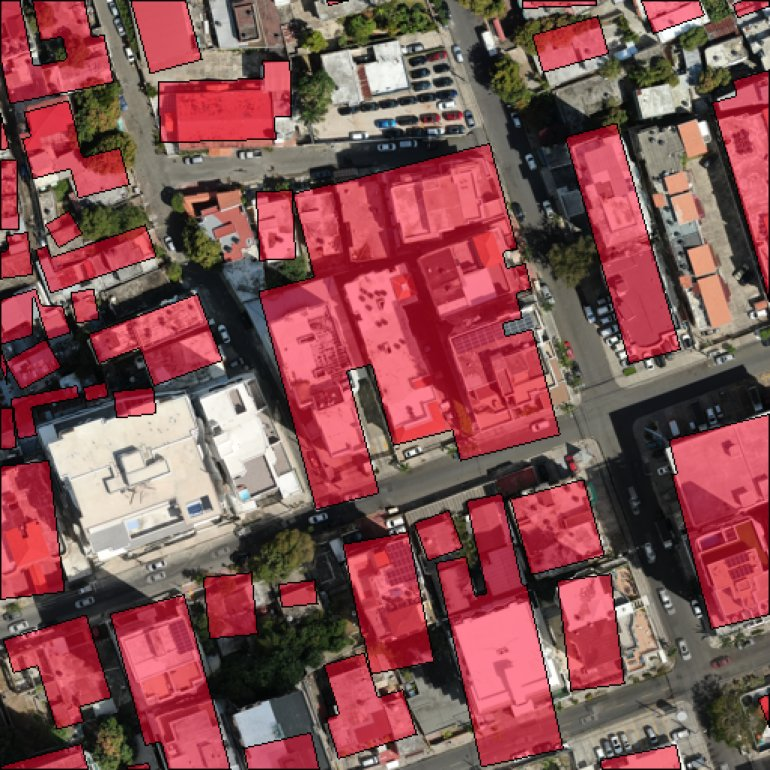
\includegraphics[width=\linewidth,height=\linewidth]{figures/santo_domingo_microsoft.jpg}
            \caption{Microsoft}
            \label{fig:sd_microsoft}
        \end{subfigure} \\
    \end{tabular}
    \caption{Three examples from the test set comparing fine-tuned Mask2Former, fine-tuned SAM2 and Microsoft GlobalMLBuildingFootprints predictions and ground truth.}
    \label{fig:test_set_examples}
\end{figure}

The evaluation results indicate that the fully automatic Mask2Former-based model achieves high accuracy using only 82 training images (tab \ref{tab:combined_eval}). An untrained Mask2Former model is incapable of building segmentation, but with minimal training data and epochs, the model achieves performance levels comparable to those in standard instance segmentation tasks \footcite{dalva_benchmarking_2024}. While the SAM2 model produces limited results without fine-tuning, its performance significantly improves with training (tab \ref{tab:combined_eval}). SAM2 performs better on shape-related metrics such as Segmentation Boundary Displacement, and its output shapes are generally sharper than those of Mask2Former.

In contrast, the Microsoft GlobalMLBuildingFootprints dataset shows poor performance in the evaluated regions (tab \ref{tab:combined_eval}). The dense and disordered arrangement of buildings in these cities is not well captured, and the dataset appears to produce reliable results only in areas with isolated, clearly defined structures.

Figure \ref{fig:test_set_examples} presents one representative tile from each of the three pilot regions, illustrating the model outputs. The corresponding quantitative evaluation results on the test set are summarized in table \ref{tab:combined_eval}. The selected evaluation metrics are standard in instance segmentation tasks and include: AJ (Aggregated Jaccard), SBD (Segmentation Boundary Displacement), PQ (Panoptic Quality), mAP (Mean Average Precision), and sAP (Sorted Average Precision) \footcite{Chen_2023_ICCV}.

\begin{table}[htbp]
\centering
\caption{Performance metrics comparison for the fine tuned models Mask2Former, SAM2 with no additional training (SAM2 base), fine-tuned SAM2 (SAM2 ft) and the Microsoft GlobalMLBuildingFootprints dataset on the test set.}
\begin{tabular}{|l|c|c|c|c|}
\hline
\textbf{Metric} & \textbf{Mask2Former} & \textbf{SAM2 base} & \textbf{SAM2 ft} & \textbf{Microsoft} \\
\hline
AJ & 0.580 & 0.554 & 0.630 & 0.099 \\
SBD & 0.560 & 0.694 & 0.737 & 0.124 \\
PQ & 0.446 & 0.477 & 0.530 & 0.002 \\
mAP & 0.224 & 0.233 & 0.277 & 0.0003 \\
sAP & 0.370 & 0.474 & 0.526 & 0.044 \\
\hline
\end{tabular}
\label{tab:combined_eval}
\end{table}

\renewcommand{\sectionnametext}{Discussion and conclusion}
\renewcommand{\headingtextR}{\thesection. \sectionnametext}
\section{\sectionnametext}

The digitalisation of building footprints remains the primary source of uncertainty within the proposed exposure workflow. To accelerate the digitalisation process, we trained and evaluated machine learning based image instance segmentation models and propose a methodology that assists humans without fully automating the task. Our findings highlight the limitations of global datasets, such as Microsoft’s Global ML Building Footprints, particularly in dense and heterogeneous urban environments. In contrast, fine-tuning task-specific models like Mask2Former and SAM2 on a small, localized dataset (82 images) led to significantly enhanced performance. Mask2Former proved effective for rapid, fully automated segmentation, whereas SAM2 demonstrated superior precision in user-assisted modes, making it well-suited for detailed refinement tasks. While human input remains essential for final evaluation and adjustments to ensure footprint accuracy, the overall workflow achieves a notable improvement in processing speed and efficiency. This represents a significant advance over previous studies, where fully automatic footprint digitalisation often resulted in low-quality outputs that had to be discarded \footcite{torres_using_2023, de_los_santos_gis-based_2021}. By combining machine learning with guided human intervention, this approach offers a practical balance between automation and reliability.


\newpage

\renewcommand{\sectionnametext}{References}
\renewcommand{\headingtextR}{\thesection. \sectionnametext}
\section{\sectionnametext}
\printbibliography[heading=none]

\end{refsection}